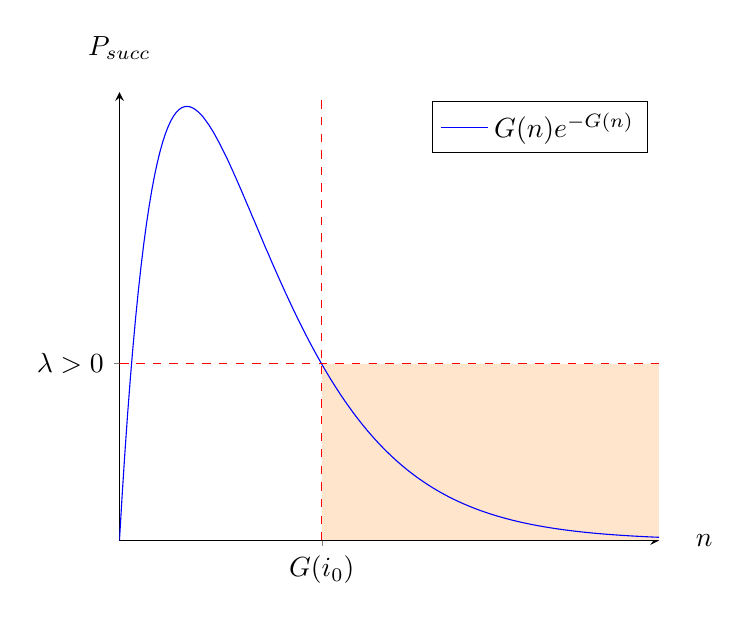
\begin{tikzpicture}
\begin{axis}[axis lines=middle,samples=200
        ,ylabel=$P_{succ}$
        ,xlabel=$n$
        ,every axis x label/.style={
          at={(ticklabel* cs:1.05)},
            anchor=west,
          },
        every axis y label/.style={
          at={(ticklabel* cs:1.05)},
            anchor=south,
          },
        ,xtick=data,
        ,xtick={0.75}
        ,xticklabels={$G(i_0)$}
        ,ytick=data,
        ,ytick={0.15}
        ,yticklabels={$\lambda>0$}
        ]
			\fill[orange!20]
				(axis cs:0.75,0) --
				(axis cs:2,0) --
				(axis cs:2,0.15) --
				(axis cs:0.75,0.15) --
				cycle;
			\addplot[blue,domain=0:2] {4*x*e^(-4*x)};
      \addplot[red,domain=0:2, dashed] {0.15};
			\addplot[red,domain=0:2, dashed] coordinates {(0.75,0) (0.75,0.38)};
			\addlegendentry{$G(n)e^{-G(n)}$}
    \end{axis}\end{tikzpicture}
